\chapter{Resolver Workflows}\label{sec:resolver-workflows}

\section{Overview}
For any scan invoked by \cxoneflow\space when \hyperref[sec:resolver-elements]{configured to use resolver}, 
a "deferred" scan is enqueued with the message queue to run a resolver scan.  The deferred scan is handed over
to a distributed resolver agent that clones the code and executes \scaresolver.  The \scaresolver results are
then sent back to the \cxoneflow endpoint server to submit for scan along with the code.  This section details
exchange, queue, and workflow logic of this process.


\section{Deferred Scan Workflow}

The \cxoneflow endpoint logs will indicate scans are deferred when the algorithm for event handling
determines a resolver scan is needed.  Figure \ref{fig:deferred-scan-flowchart} shows the deferred-scan
workflow algorithm that is followed to determine when to request a deferred scan.  

\begin{figure}[ht]
  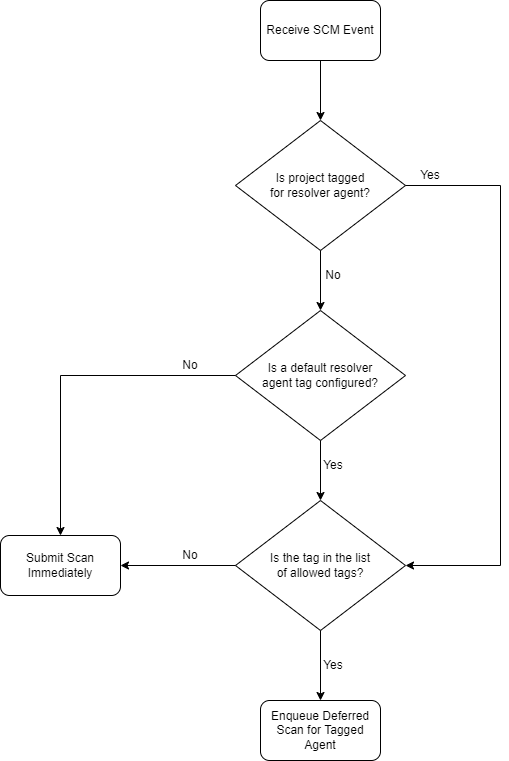
\includegraphics[width=\textwidth]{graphics/cxoneflow-diagrams-Deferred Scan Algorithm.png}
  \caption{Deferred Scan Algorithm}
  \label{fig:deferred-scan-flowchart}
\end{figure}


\section{Post Deferred Scan Workflow}

When the \scaresolver scan is complete, the distributed resolver agent will send the results
to the \cxoneflow endpoint for submission in the \cxone scan.  Scans with \scaresolver can
complete successfully or end with failure.

If the \scaresolver scan is successful, the results of the 
\href{https://docs.checkmarx.com/en/34965-19199-running-scans-using-checkmarx-sca-resolver.html#UUID-af718204-6dfc-2b27-439e-419b9157d364_id_RunningScansUsingCheckmarxSCAResolver-CheckmarxSCAResolverModes}{offline}
scan are submitted as part of the \cxone scan.  If the \scaresolver scan fails (for any reason), the \cxone scan is submitted for server-side dependency resolution.
Figure \ref{fig:post-deferred-scan-flowchart} shows the post-deferred-scan workflow algorithm.

\begin{figure}[ht]
  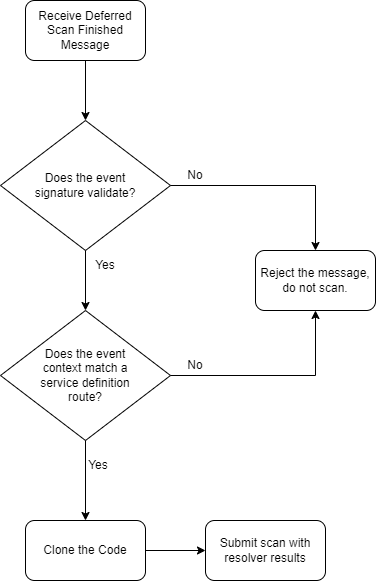
\includegraphics[width=\textwidth]{graphics/cxoneflow-diagrams-Post Deferred Scan Algorithm.png}
  \caption{Post Deferred Scan Algorithm}
  \label{fig:post-deferred-scan-flowchart}
\end{figure}



